\section{Problem 5: Two-Period Portfolio Choice}

The consumer lives for two periods and has Epstein--Zin preferences
\begin{equation}
  V(m) =
  \left[
    c_1^{1-\gamma}
    + \beta
    \left(\E\, c_2^{1-\sigma}\right)^{\frac{1-\gamma}{1-\sigma}}
  \right]^{\frac{1}{1-\gamma}},
  \label{eq:p5-ez}
\end{equation}
where $\gamma$ is inverse EIS and $\sigma$ is risk aversion. The consumer begins period 1 with cash-on-hand $m>0$ and chooses (i) the savings share $x \ge 0$ and (ii) the risky share of savings $x_s \in [0,1]$ (no borrowing, no short-selling). Period-1 consumption is
\begin{equation}
  c_1 = (1-x)m.
\end{equation}
The consumer can invest savings $xm$ in a safe asset with gross return $R_f = 1+r$ or a risky asset with gross return $R = 1+r+\varepsilon_2$. Period-2 consumption is
\begin{equation}
  c_2 = y_2 + (1+r)xm + \varepsilon_2 x_s xm.
  \label{eq:p5-c2}
\end{equation}
The pair $(\log y_2,\varepsilon_2)$ is jointly normal:
\begin{equation}
  \begin{bmatrix}\log y_2 \\ \varepsilon_2\end{bmatrix}
  \sim \mathcal{N}\left(
  \begin{bmatrix}0 \\ \mu\end{bmatrix},
  \begin{bmatrix}
    \sigma_y^2 & \rho \sigma_y \sigma_\varepsilon \\
    \rho \sigma_y \sigma_\varepsilon & \sigma_\varepsilon^2
  \end{bmatrix}
  \right).
\end{equation}
We solve the problem for two correlations, $\rho \in \{0.3,0.6\}$.

\paragraph{Parameters.}
We use $\beta = 0.90$, $\sigma = 5$, $\gamma = 1/2$, $r = 0.04$, $\mu = 0.06$, $\sigma_\varepsilon = 0.15$, and $\sigma_y = 0.20$. We solve for a grid of cash-on-hand values $m \in [0.1,10]$.

\subsection{Optimality conditions and Euler equations}

Define the period-2 certainty equivalent
\begin{equation}
  CE_2 \equiv \left(\E\,c_2^{1-\sigma}\right)^{\frac{1}{1-\sigma}}.
\end{equation}
Since the outer power in \eqref{eq:p5-ez} is monotone, the choice problem is equivalent to maximizing
\begin{equation}
  J \equiv c_1^{1-\gamma} + \beta CE_2^{1-\gamma}.
\end{equation}
Let the stochastic discount factor associated with these preferences be
\begin{equation}
  M_2
  \equiv
  \left(\frac{c_2}{c_1}\right)^{-\gamma}
  \left(\frac{c_2}{CE_2}\right)^{\gamma-\sigma}.
  \label{eq:p5-sdf}
\end{equation}
At an interior optimum, the Euler equations for the safe and risky assets are
\begin{align}
\begin{split}
  1 &= \beta\,\E\left[ M_2 (1+r) \right],\\
  1 &= \beta\,\E\left[ M_2 (1+r+\varepsilon_2) \right].
\end{split}\label{eq:p5-euler}
\end{align}
These are the equations we use for diagnostic checks. When the constraints bind (e.g.\ $x=0$ or $x_s \in \{0,1\}$), the corresponding Euler equation need not hold with equality.

\subsection{Numerical solution}

\subsubsection{Quadrature for $(\log y_2,\varepsilon_2)$}

We approximate expectations with tensor-product Gauss--Hermite quadrature. This choice is natural because $(\log y_2,\varepsilon_2)$ is bivariate normal: Gauss--Hermite quadrature is designed for integrals with a Gaussian (normal) weight function, and the multivariate version uses a tensor product of one-dimensional Gauss--Hermite rules, matching the joint normal density.

The integrand $g(y_2,\varepsilon_2)$ in the quadrature is the object whose expectation we need. For the Euler equations \eqref{eq:p5-euler} this is the stochastic discount factor times the asset's gross return: $g = M_2 \times \text{(gross return)}$. The SDF $M_2$ depends on $(y_2,\varepsilon_2)$ through period-2 consumption $c_2 = y_2 + (1+r)xm + \varepsilon_2 x_s xm$. Concretely, for the safe-asset equation we use $g_{\text{safe}}(y_2,\varepsilon_2) = M_2(y_2,\varepsilon_2)\,(1+r)$; for the risky-asset equation we use $g_{\text{risky}}(y_2,\varepsilon_2) = M_2(y_2,\varepsilon_2)\,(1+r+\varepsilon_2)$. With nodes $\{(\log y_2^j,\varepsilon_2^j)\}_{j=1}^J$ and weights $\{w_j\}_{j=1}^J$ (with $\sum_j w_j=1$), we set $y_2^j = \exp(\log y_2^j)$ and approximate
\begin{equation}
  \E[g(y_2,\varepsilon_2)] \approx \sum_{j=1}^J w_j\, g(y_2^j,\varepsilon_2^j).
\end{equation}
We use $7$ nodes in each dimension (so $J=49$). 

\subsubsection{Optimization over $(x,x_s)$}

For each $m$ and each $\rho$, we solve the bounded two-dimensional maximization problem
\begin{equation}
  \max_{x\in[0,1],\,x_s\in[0,1]} \; V(m;x,x_s),
\end{equation}
where $V$ is defined by \eqref{eq:p5-ez}--\eqref{eq:p5-c2}. We solve via a bounded quasi-Newton optimizer (L-BFGS-B) on $-V$, using \texttt{hetmacro.optimize.minimize\_lbfgsb}.

\begin{algorithm}[H]
\caption{Solve policies for each $m$ and $\rho$}
\label{alg:p5-solve}
\begin{algorithmic}[1]
\State \textbf{Input:} $m$ grid, parameters $p$, correlation $\rho$
\State \textbf{Output:} policy functions $x(m)$ and $x_s(m)$
\State Build quadrature nodes/weights for $(\log y_2,\varepsilon_2)$
\For{each $m$}
  \State Solve $\max_{x,x_s\in[0,1]} V(m;x,x_s)$ via L-BFGS-B
\EndFor
\State \textbf{return} $x(m)$, $x_s(m)$
\end{algorithmic}
\end{algorithm}

\subsection{Results and Euler diagnostics}

\Cref{fig:p5-policies} plots the optimal saving share $x(m)$ and risky share $x_s(m)$ for $\rho=0.3$ and $\rho=0.6$. \Cref{fig:p5-euler} shows Euler residuals for the safe and risky asset, computed from \eqref{eq:p5-euler} and masked to points where both controls are interior (away from the bounds).

\begin{figure}[H]
\centering
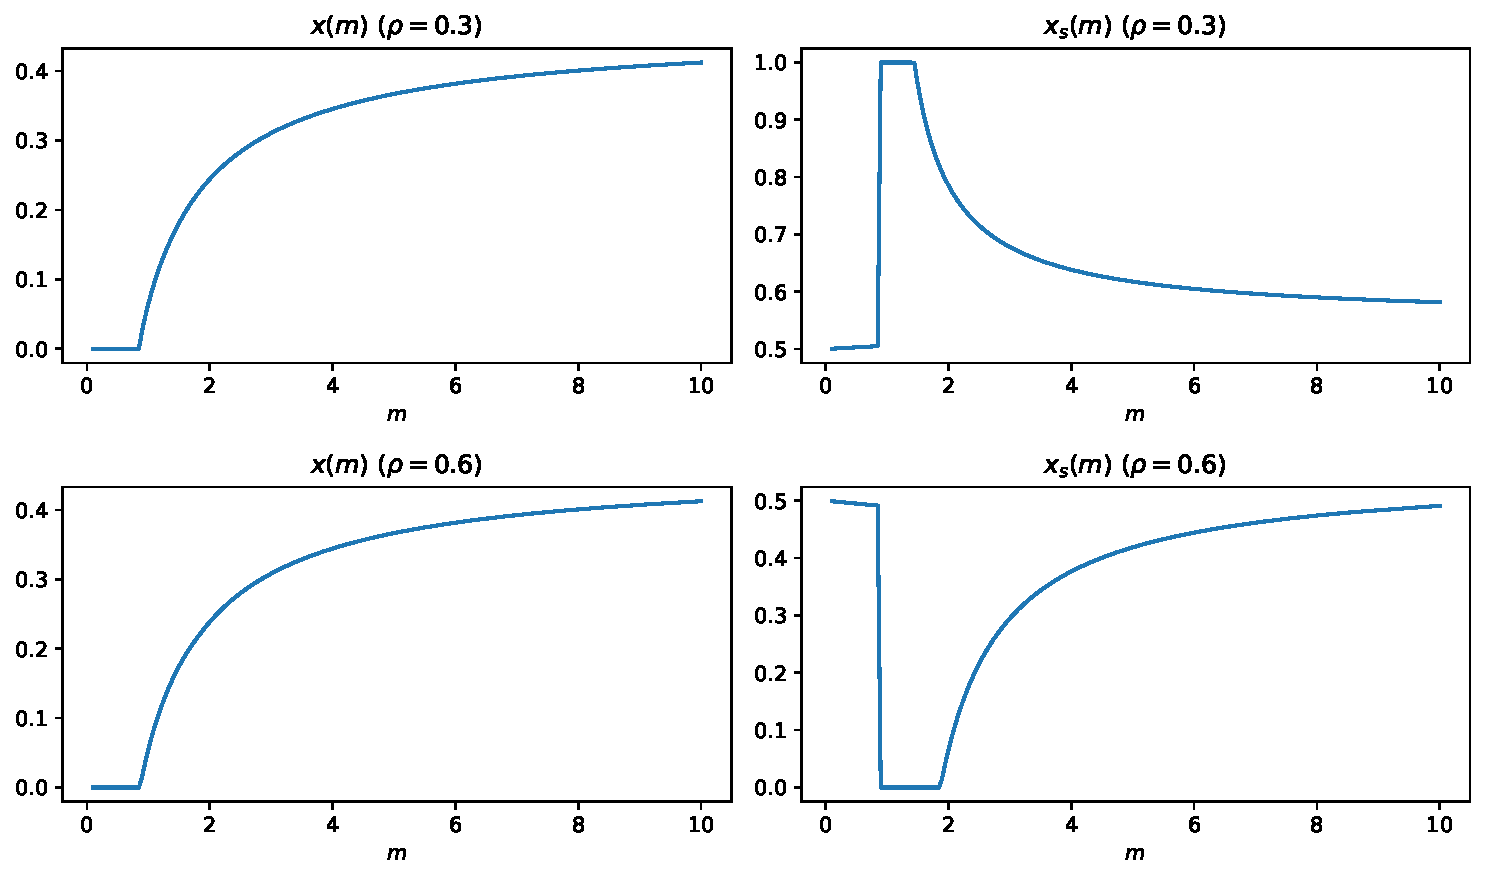
\includegraphics[width=0.95\textwidth]{figures/problem5_policies}
\caption{Problem 5 policy functions: saving share $x(m)$ and risky share $x_s(m)$ for correlations $\rho=0.3$ and $\rho=0.6$.}
\label{fig:p5-policies}
\end{figure}

\begin{figure}[H]
\centering
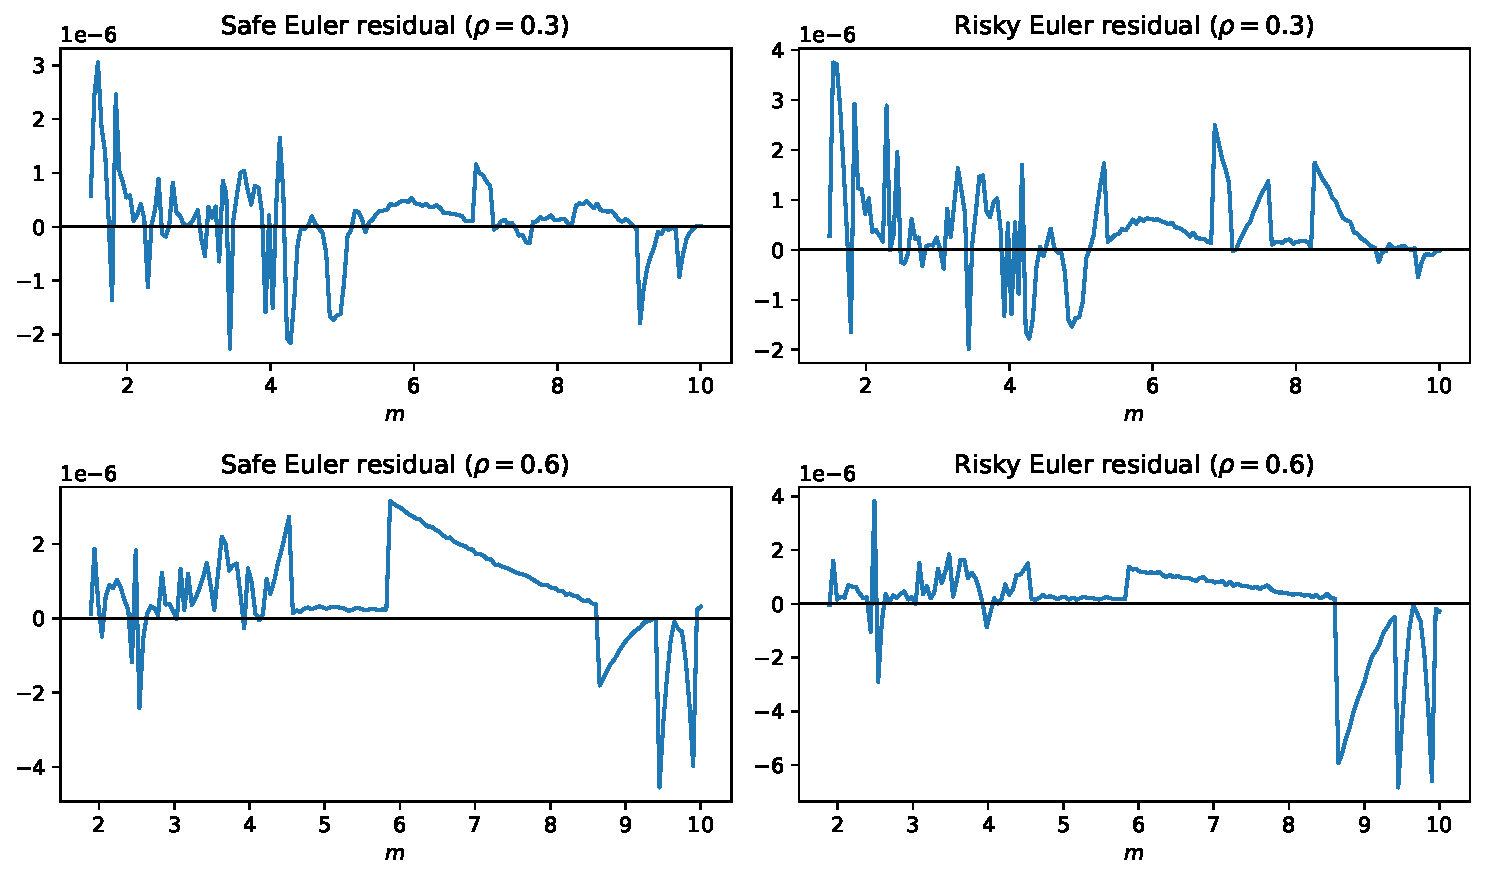
\includegraphics[width=0.95\textwidth]{figures/problem5_euler_residuals}
\caption{Euler residual diagnostics for the safe and risky asset, computed using the Epstein--Zin SDF \eqref{eq:p5-sdf} and masked to (approximate) interior points where $x\in(0,1)$ and $x_s\in(0,1)$.}
\label{fig:p5-euler}
\end{figure}

